\section{Differential Privacy Definition}


\begin{definition}(\(\epsilon\)-Differential Privacy \cite{dwork2006differential})
Given a privacy parameter \(\epsilon \geq 0\), for any two adjacent inputs \(x, x' \in X\) and each potential output \(y \in Y\), a randomized mechanism \(M\) satisfies \(\epsilon\)-differential privacy (DP) if it ensures that
\[
\frac{\Pr[M(x) = y]}{\Pr[M(x') = y]} \leq e^{\epsilon}.
\]
\end{definition}


\section{SanText and CusText}

\subsection{SanText}


Below, we detail the operational steps of the token sanitization mechanism \( M \) of SanText when processing an input token \( x \):

\begin{enumerate}
    \item \( M \) is parameterized by the privacy parameter \( \epsilon \) and employs a metric $d$ to measure distances between tokens.
    \item The utility function \( u \) is defined such that \( u(x, x) = -d(x, x) \). Under this definition, \( M \) selects an output from \( Y \) based on the exponential mechanism (Def.~\ref{def:expmech}) tailored for the specified \( \epsilon \), but with the utility sensitivity \( \Delta u \) replaced by \( 1 \).
\end{enumerate}

\subsection{CusText}

We describe CusText's token sanitization algorithm $M:X'\rightarrow X$ for input token $x$. 

\begin{enumerate}
    \item $M$ is parametrized by the formed clusters, a distance $d$, and the privacy parameter $\epsilon$.
    \item Let $C\subseteq X$ be the cluster $x$ belongs in.
    \item Let utility $u:C \times C \rightarrow \mathbb{R}$ be the negative of the normalised distance $u(x,y) = - \frac{d(x,y) - d_{\min}}{d_{\max} - d_{\min}}$ ($d_{\min} = \min_{x,y\in C}d(x,y)$ and $d_{\max}= \max_{x,y\in C}d(x,y)$), so that sensitivity $\Delta u = 1$. 
    \item Using the above utility function, replace $x$ with some token in $C$ via the exponential mechanism (Def.~\ref{def:expmech}) for privacy $\epsilon$.
\end{enumerate}

We present the proof that CusText cannot achieve standard (M)LDP when there is more than one cluster.
\begin{proof}
    We prove first for LDP.  Suppose for contradiction that there exists $\epsilon\in \mathbb{R}$ such that $M$ satisfies $\epsilon$-LDP. Then for all $x, x' \in X', y \in X$, this inequality must hold: 
    $$
        \Pr(M(x) = y) \leq e^\epsilon \Pr(M(x') = y)
    $$
    Since there are at least two clusters, there must exist $x, x' \in X'$ that belong in different clusters. Let $y$ be a token in the cluster of $x$, which means $y$ is not in the cluster of $x'$. This means that $\Pr(M(x) = y) > 0$ and $e^\epsilon \Pr(M(x') = y) = e^\epsilon \cdot 0 = 0$. Thus the above inequality cannot hold, which is a contradiction, and thus there is no  $\epsilon$ for which $M$ is $\epsilon$-LDP.

     The proof for metric LDP follows since if $M$ is $\epsilon$-metric LDP then  $M$ is $\epsilon\cdot \Delta u$-LDP. Since the lexicon is finite, $\Delta u$ maximises over a finite set and is also finite. Thus, if $M$ is $\epsilon$-metric LDP then it is $\epsilon'$-LDP for some finite $\epsilon'$ (which we just proved is impossible).    
\end{proof}


\section{Detailed Experimental Results}

Here we give the detailed prompt for obtaining the extended set $X'$ of sensitive tokens using GPT-4o.

{\em
\begin{quote}
If I give you a word or phrase, example ``southern norrland,'' can you give me 100 similar words/phrases of the same category?

For example:
\begin{itemize}
    \item If it is a location, give me other locations that are similar in nature.
    \item If it is an organization, give me other organizations that are similar.
    \item If it is an object, give me other objects that are similar.
\end{itemize}

The similarity should be in terms of the category and characteristics of the entity. The words you give should make sense if used as a replacement for the original word/phrase in a similar context.

Format output as a list of words/phrases:
\[
[\text{word/phrase1, word/phrase2, ...}]
\]

Here the context that "\{search\_phrase\}" was used in: "\{context\}".
\end{quote}
}


For example, when the search phrase was `sarpsborg city court (tingrett)' with its context in the TAB text, the output we received from GPT-4o was:

[`oslo district court', `bergen district court', `trondheim district court', `stavanger district court', `kristiansand district court', `tromsø district court', `drammen district court', `fredrikstad district court', `skien district court', `ålesund district court', `bodø district court', `hamar district court', `molde district court', `haugesund district court', etc].


Now we give detailed experimental results on 
semantic similarity (Figure~\ref{fig:semsim}),
perplexity (Figure~\ref{fig:perplexity}),
grammar (Figure~\ref{fig:grammar}),
common sense (Figure~\ref{fig:common_sense}), 
coherence (Figure~\ref{fig:coherence}), and 
cohesiveness (Figure~\ref{fig:cohesiveness}).
For perplexity we used GPT-2. To judge the grammar, common sense, coherence, and cohesiveness of santized text, we used GPT-4o, with the following prompt. 


{\em
\begin{quote}
Could you please evaluate the following passage for its grammar, common sense, coherence, and cohesiveness? Score it on a scale from 1 to 5, where 1 is the lowest (poor quality) and 5 is the highest (excellent quality).

You should score based on these criteria:
\begin{itemize}
    \item \textbf{Grammar}: Are the sentences structured correctly?
    \item \textbf{Common sense}: Does the content make logical sense in the real world?
    \item \textbf{Coherence}: Do the ideas flow logically from one sentence to another?
    \item \textbf{Cohesiveness}: Do all parts of the text come together in a unified whole?
\end{itemize}

Please ONLY respond in JSON format with the four keys 'grammar', 'common sense', 'coherence', and 'cohesiveness', each with a score attached to them.
\end{quote}
}


CluSanT's improvement over SanText generally increases with the number of clusters used. Increasing the number of clusters and parameter \(k\) significantly enhances CluSanT’s performance, approaching that of CusText. Although CusText performs better across metrics, it offers weaker privacy guarantees. Note that these metrics represent general trends, and due to noisy judgments from LLMs, smaller \(k\) values can sometimes yield better results.



\begin{figure*}
    \centering
    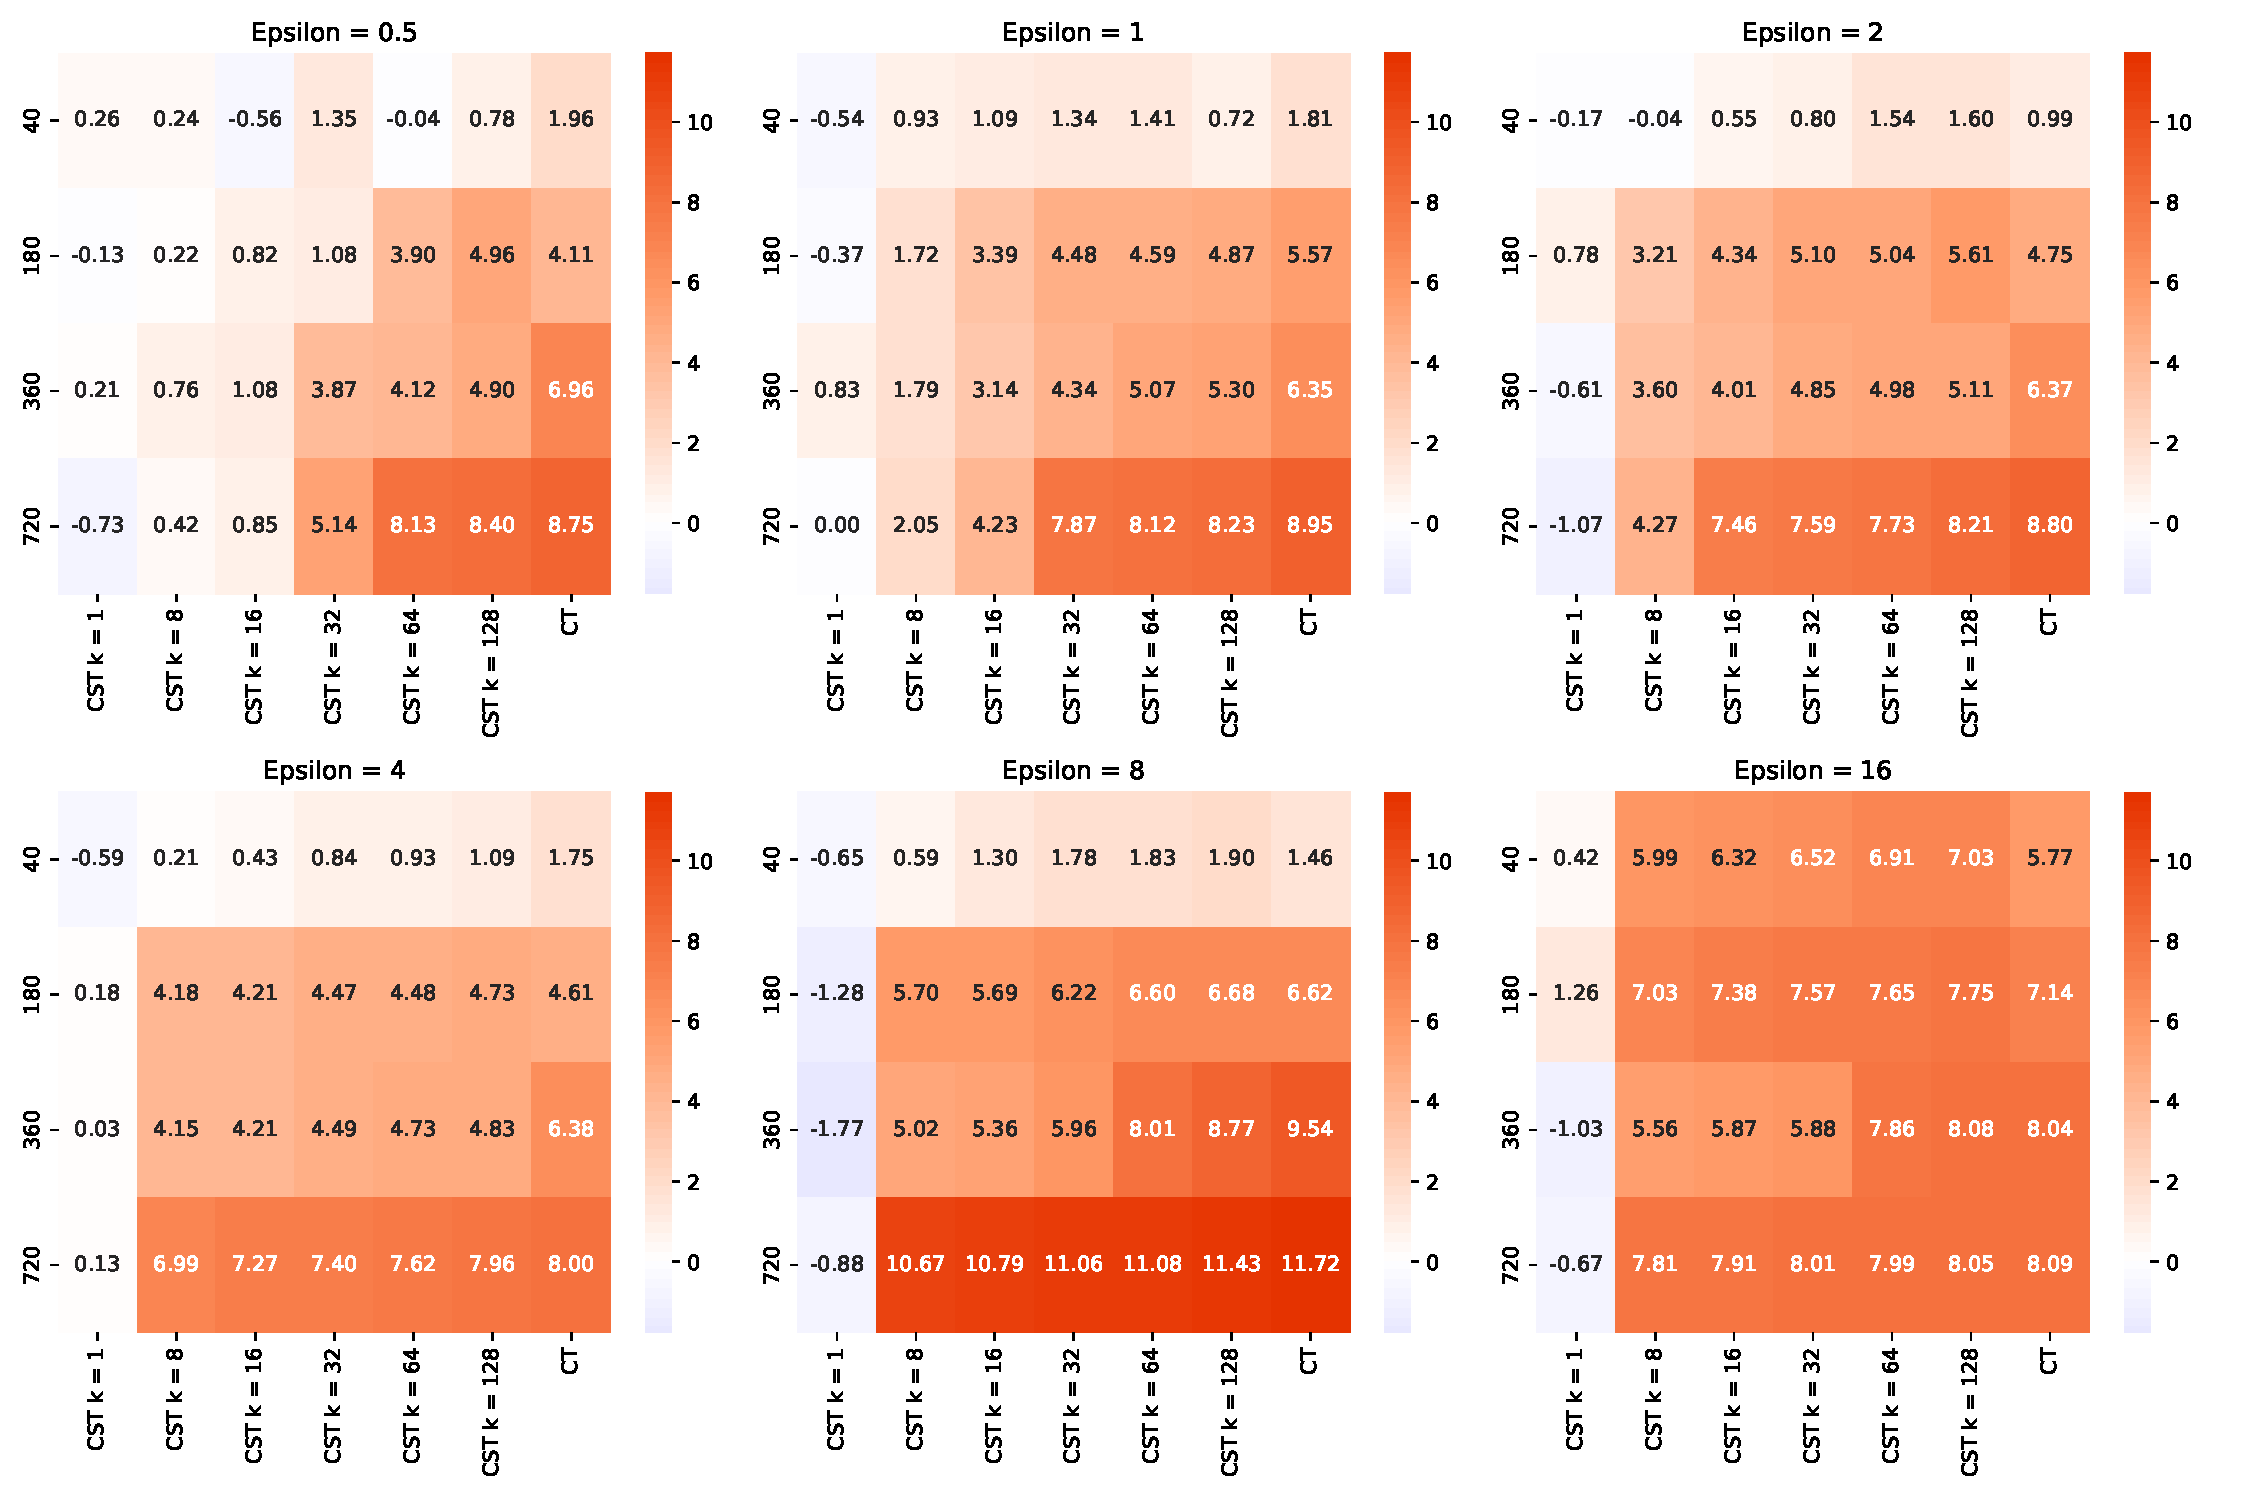
\includegraphics[width=15cm]{fig/heatmap_semantic_sim.pdf}
    \caption{Semantic similarity improvement over SanText (\%); the higher, the better. \clusant abbr. by CST and CusText by CT. Horizontal axis varies parameter $k$ of \clusant. Vertical axis varies the number of clusters. Same axes apply for the other heatmaps as well.}
    \label{fig:semsim}
\end{figure*}


\begin{figure*}
    \centering
    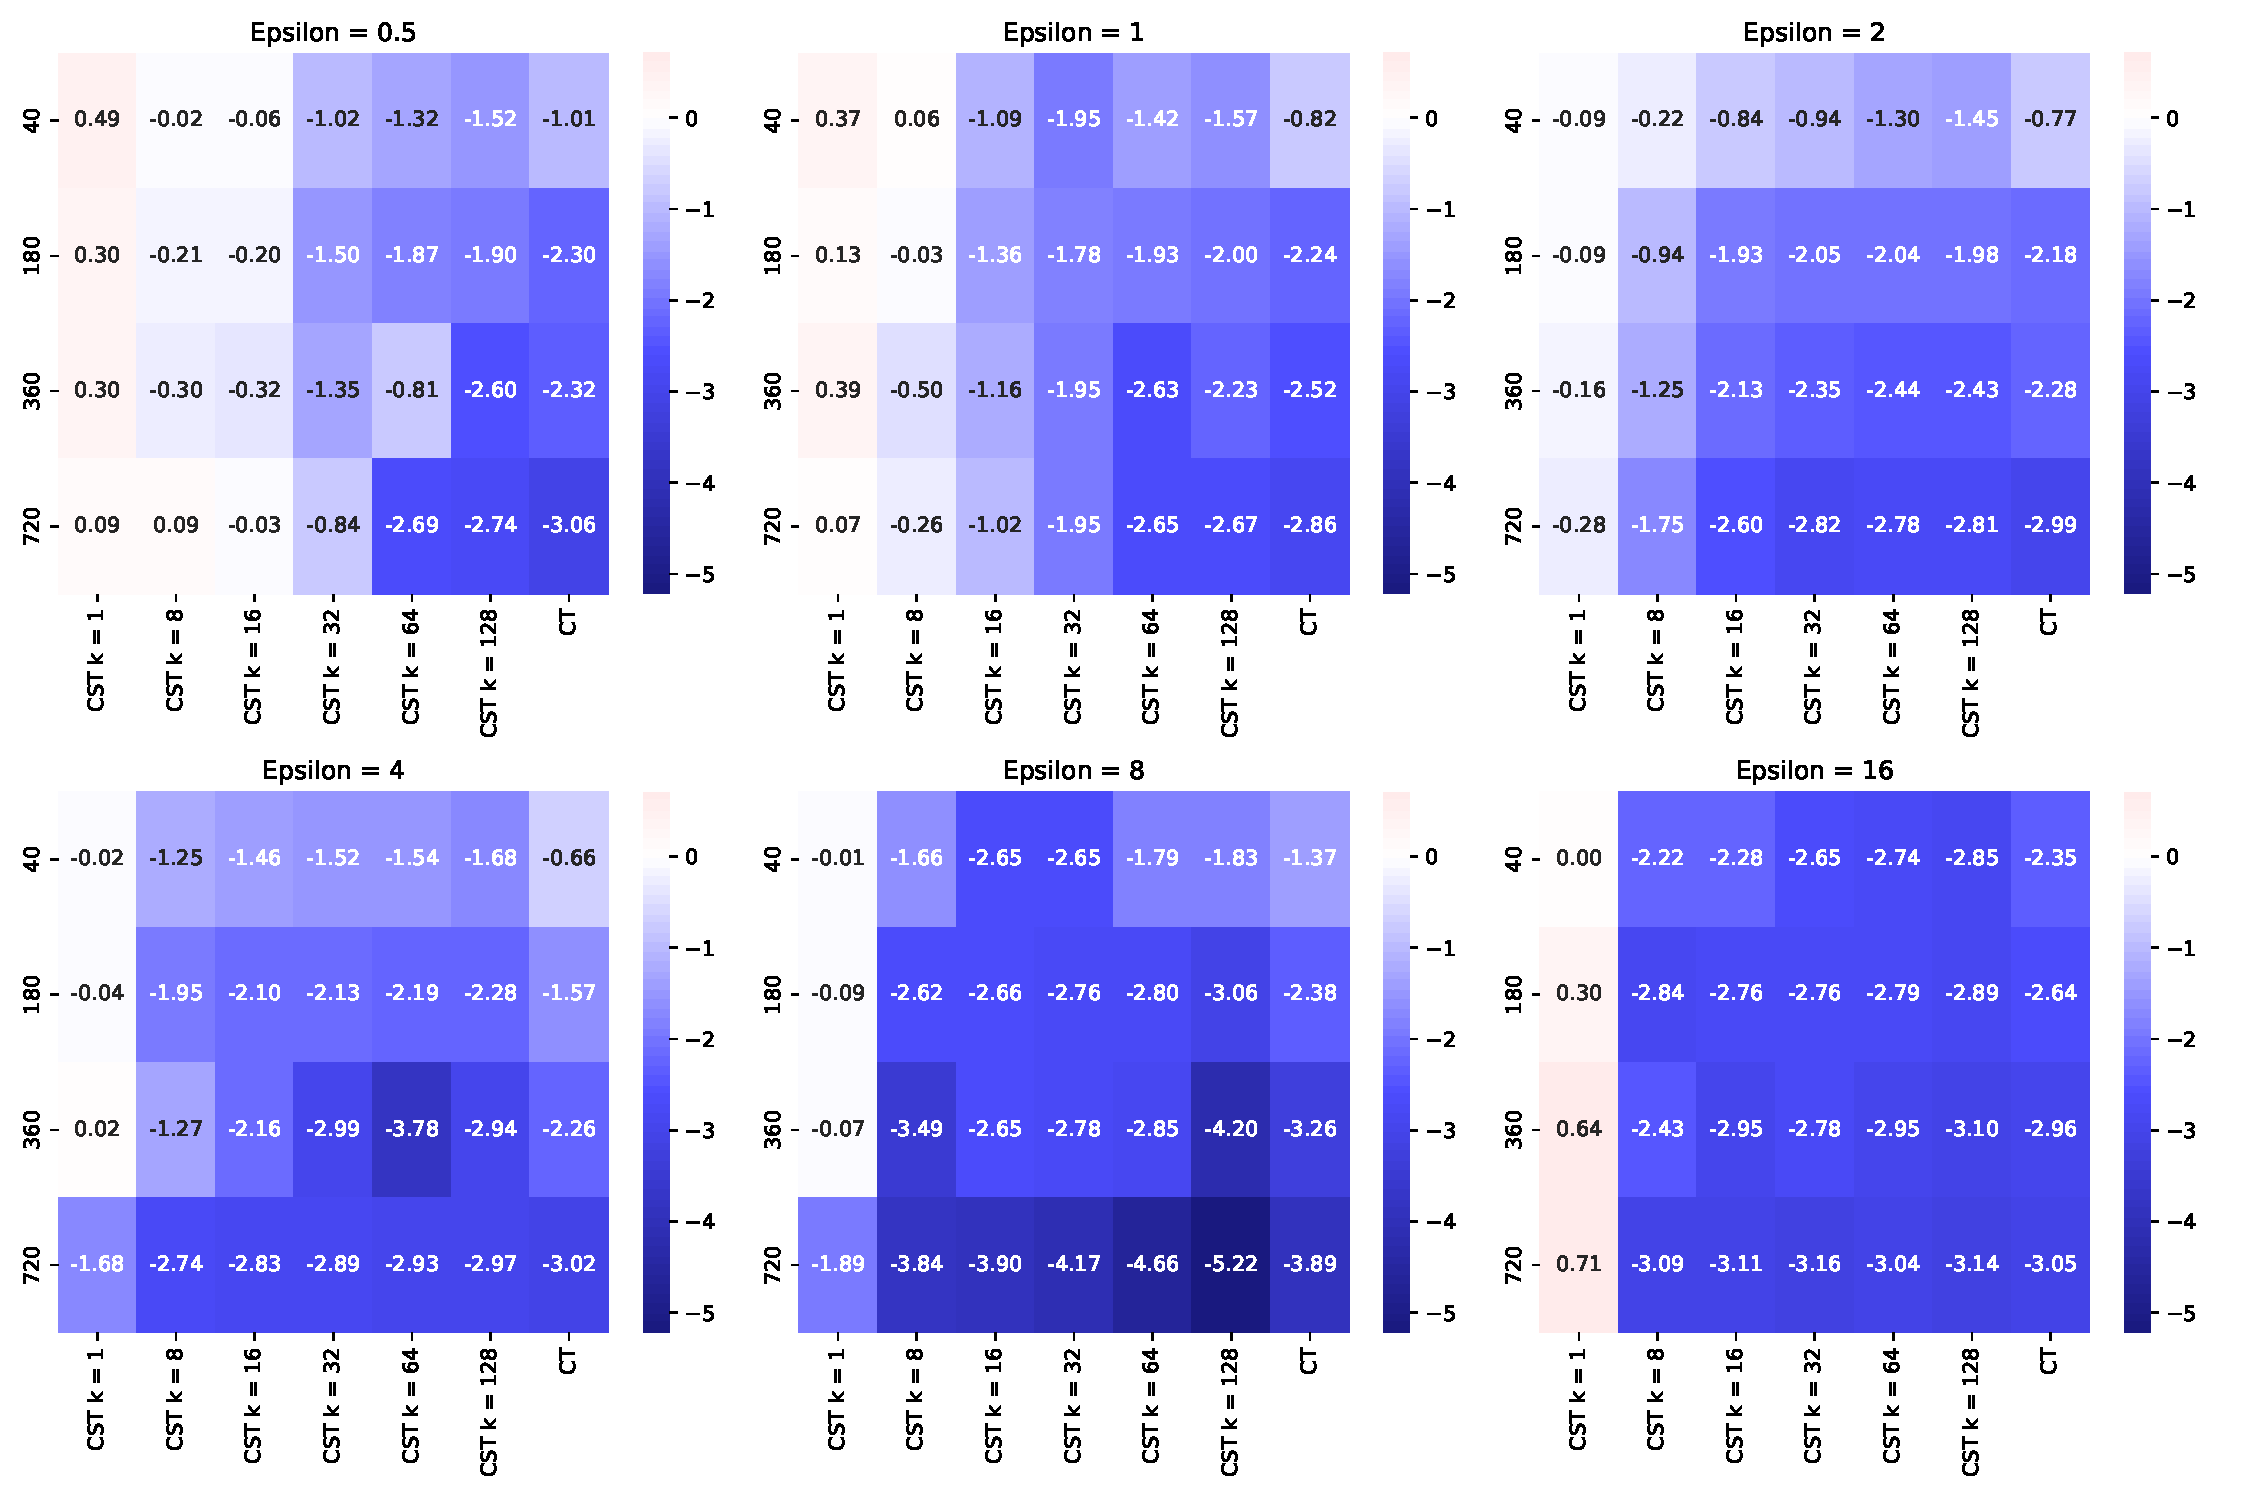
\includegraphics[width=15cm]{fig/heatmap_perplexity.pdf}
    \caption{Peplexity improvement over SanText (\%); the lower, the better.}
    \label{fig:perplexity}
\end{figure*}



\begin{figure*}
    \centering
    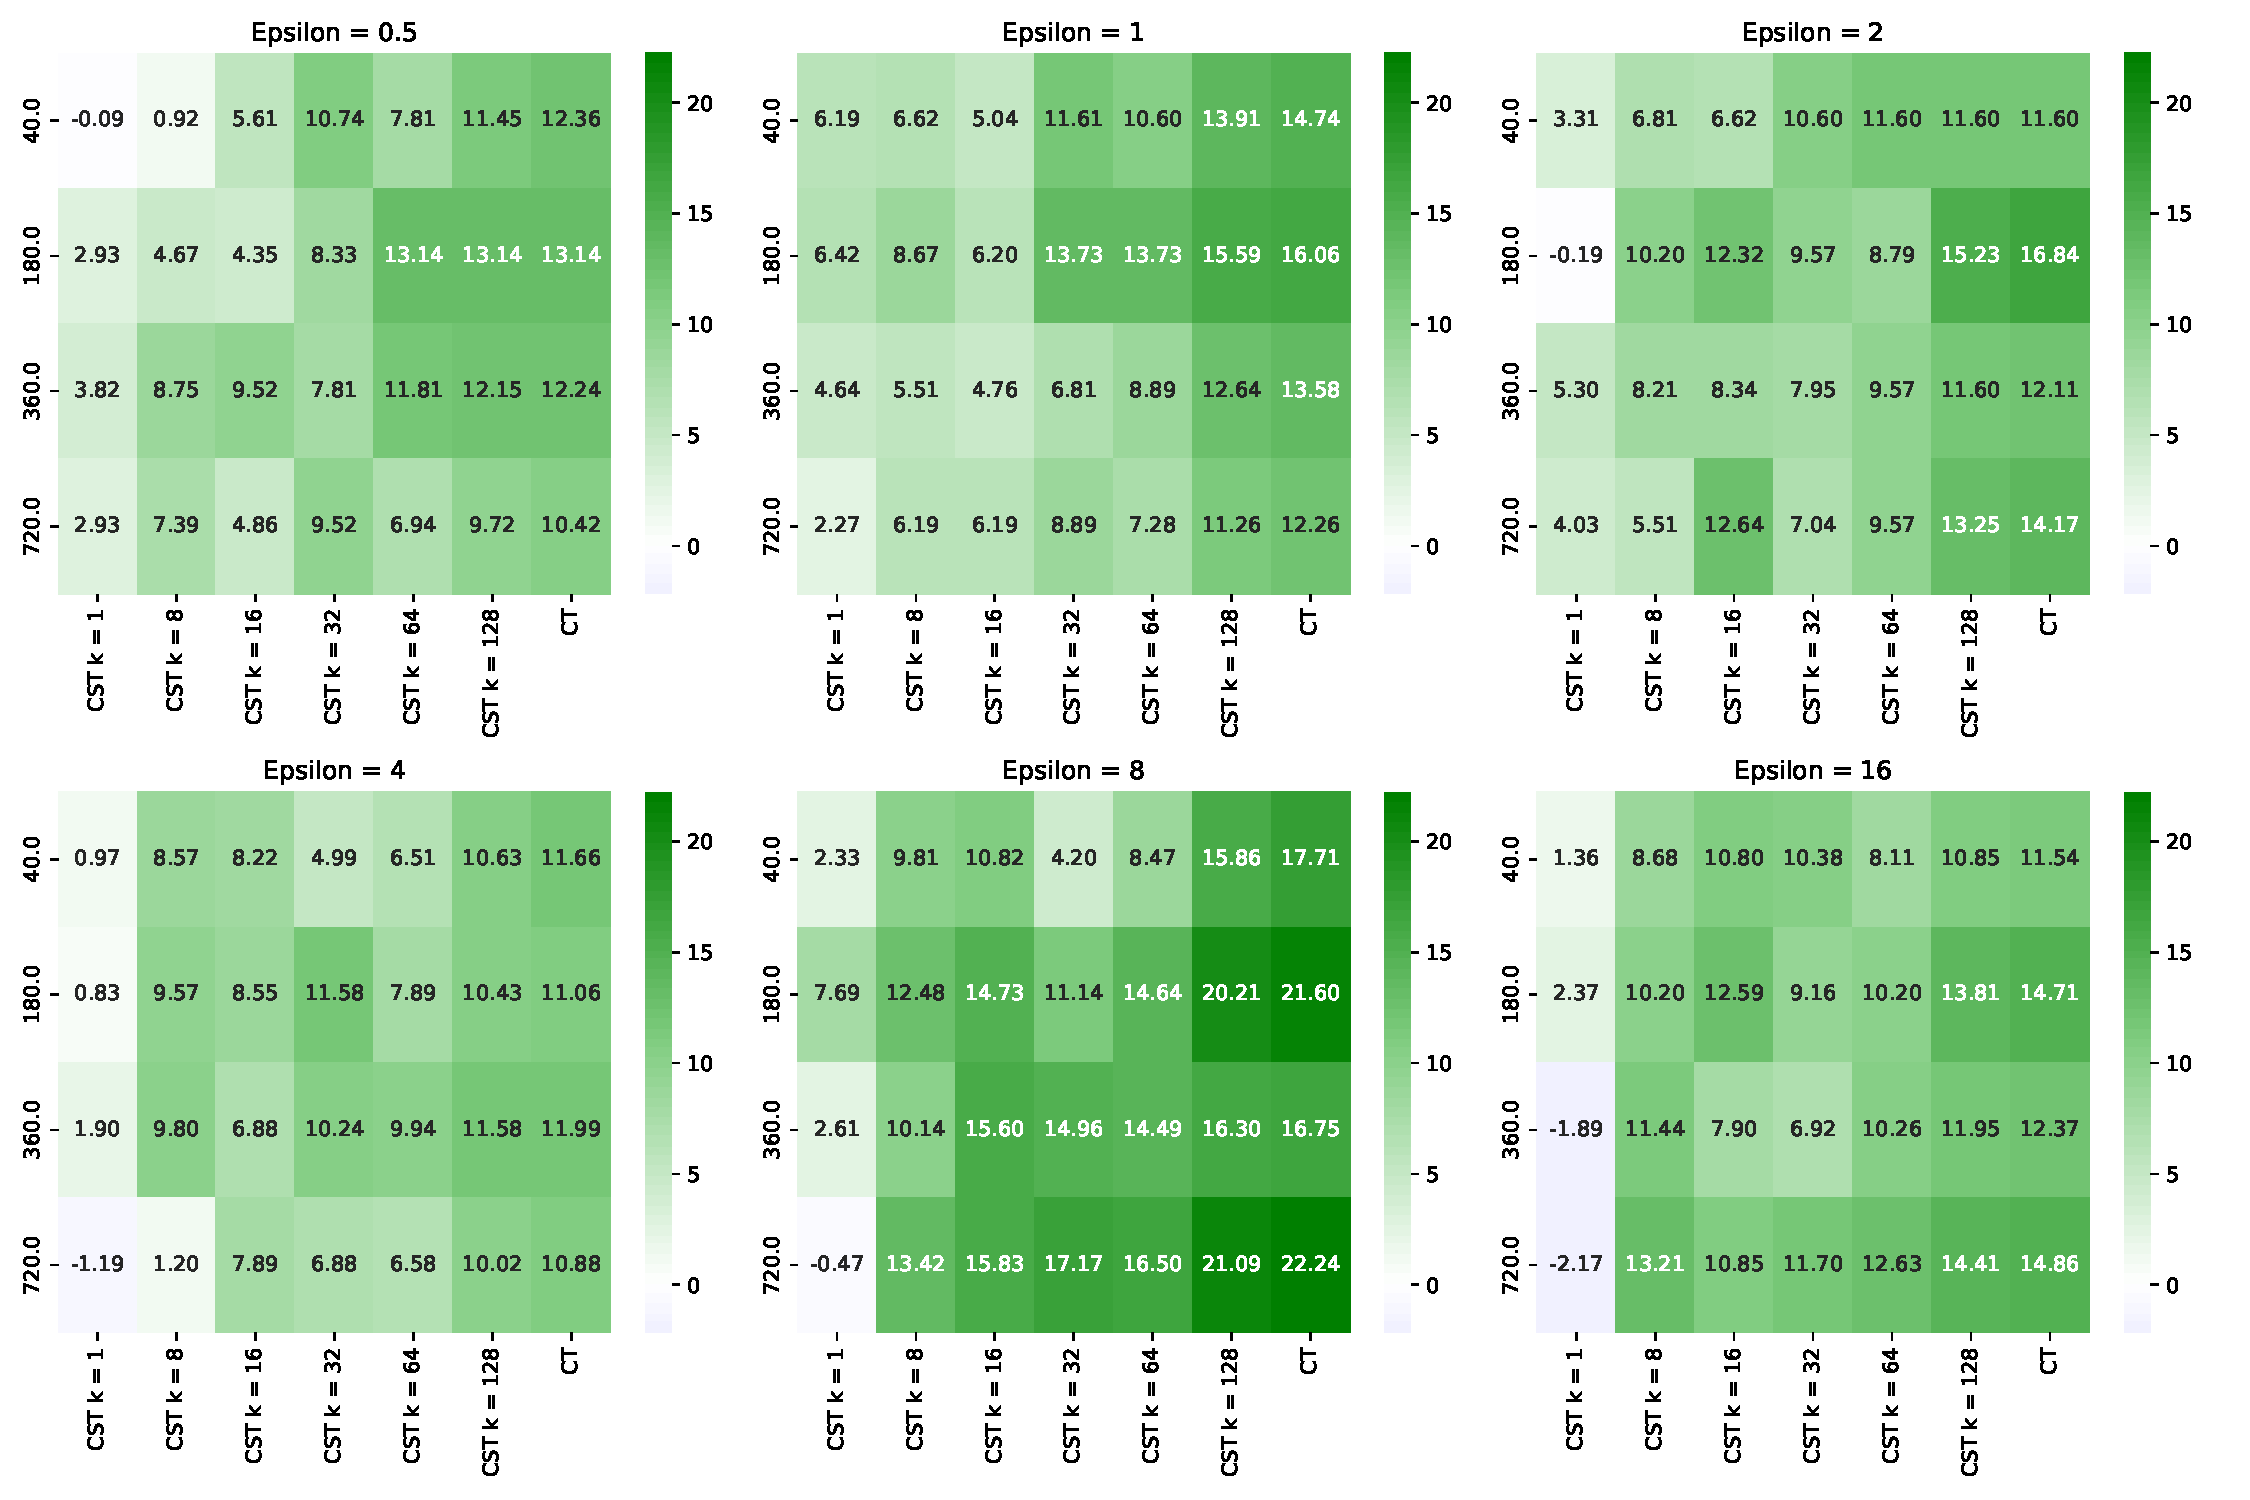
\includegraphics[width=15cm]{latex/fig/heatmap_grammar.pdf}
    \caption{Grammar improvement over SanText (\%); the higher, the better.}
    \label{fig:grammar}
\end{figure*}


\begin{figure*}
    \centering
    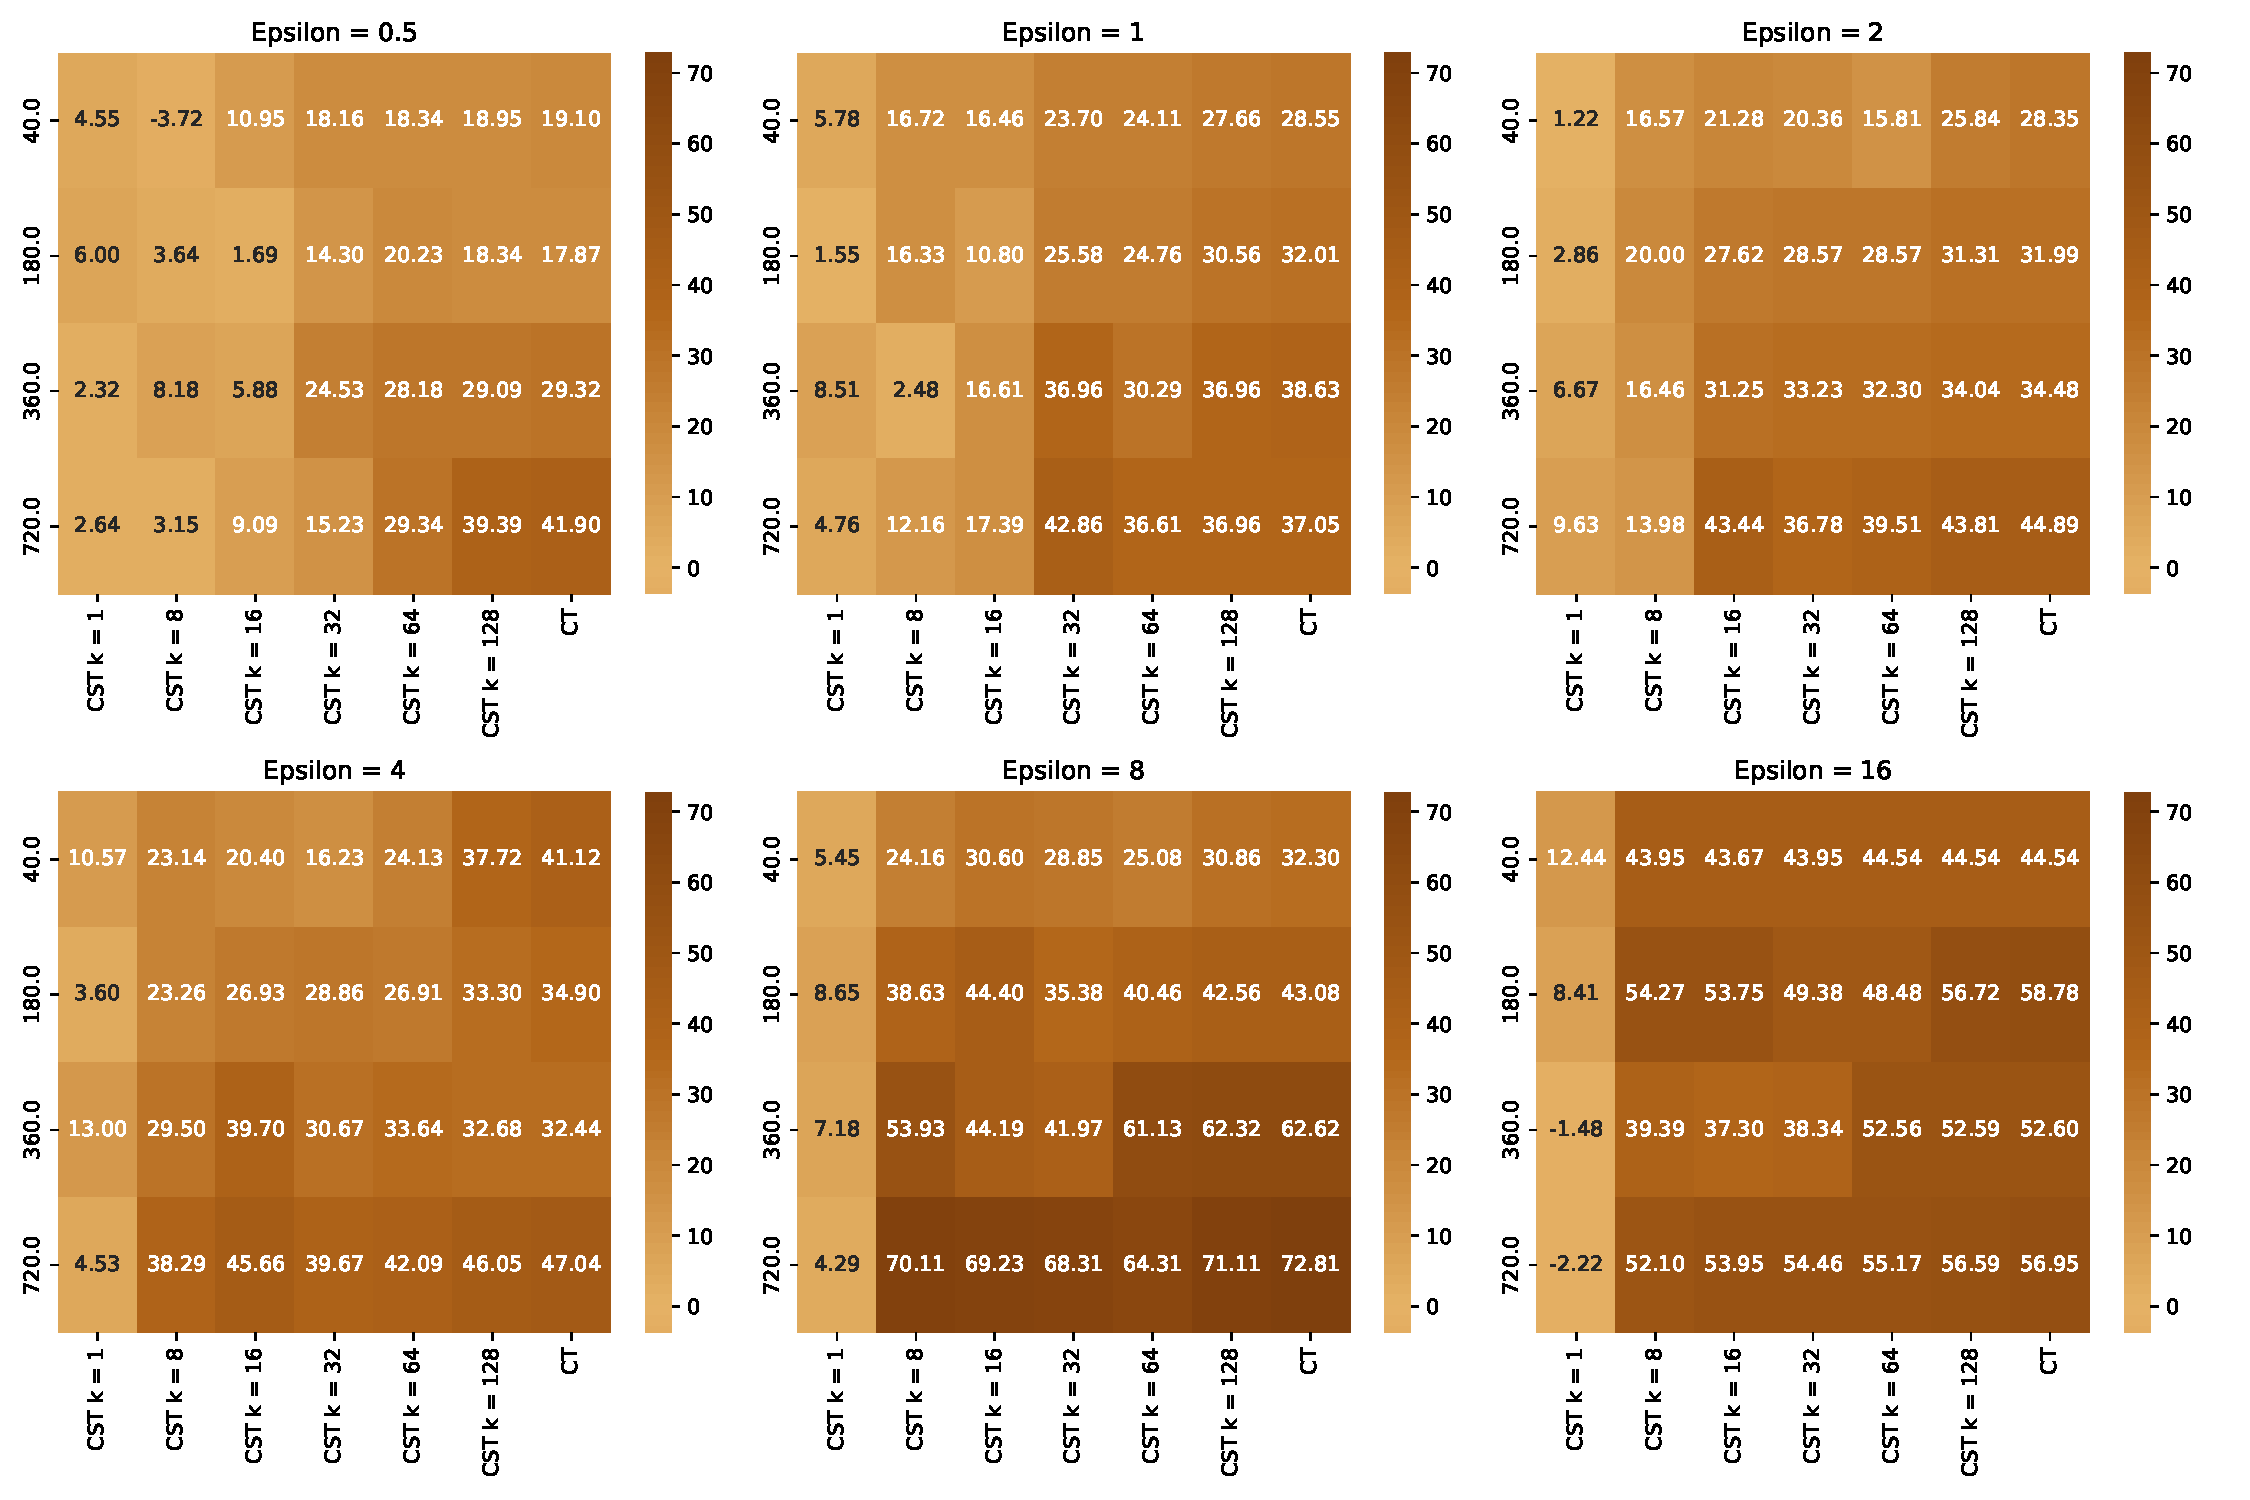
\includegraphics[width=15cm]{latex/fig/heatmap_common_sense.pdf}
    \caption{Common Sense improvement over SanText (\%); the higher, the better.}
    \label{fig:common_sense}
\end{figure*}


\begin{figure*}
    \centering
    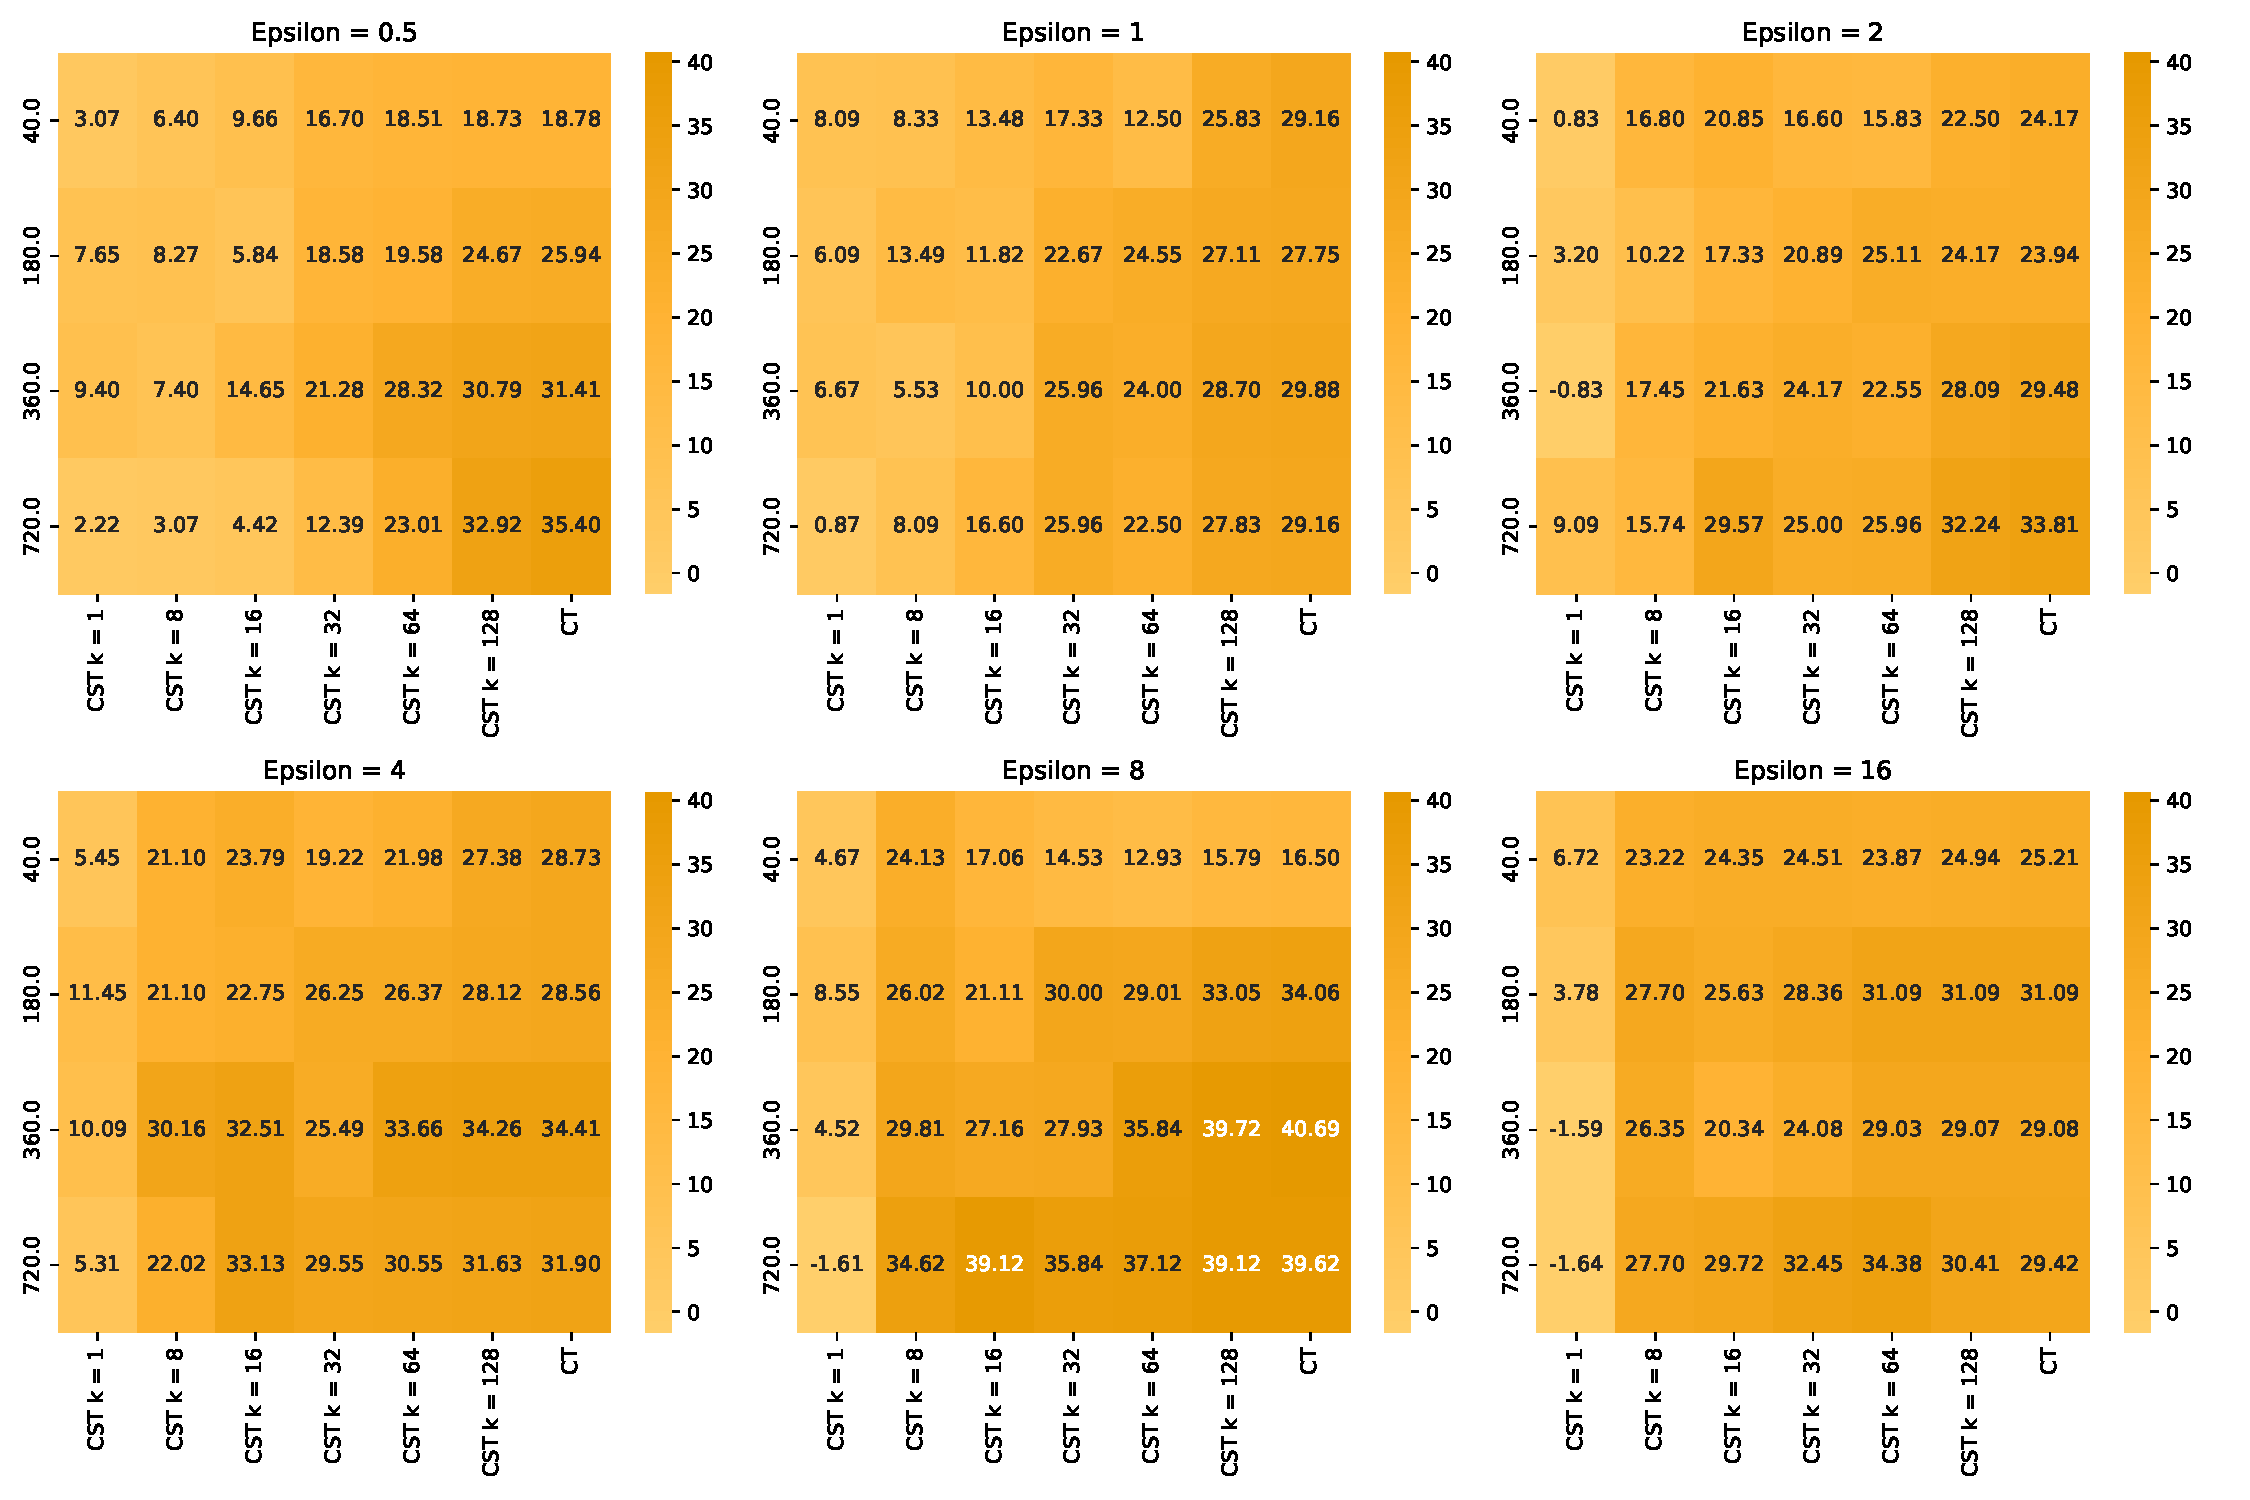
\includegraphics[width=15cm]{latex/fig/heatmap_coherence.pdf}
    \caption{Coherence improvement over SanText (\%); the higher, the better.}
    \label{fig:coherence}
\end{figure*}


\begin{figure*}
    \centering
    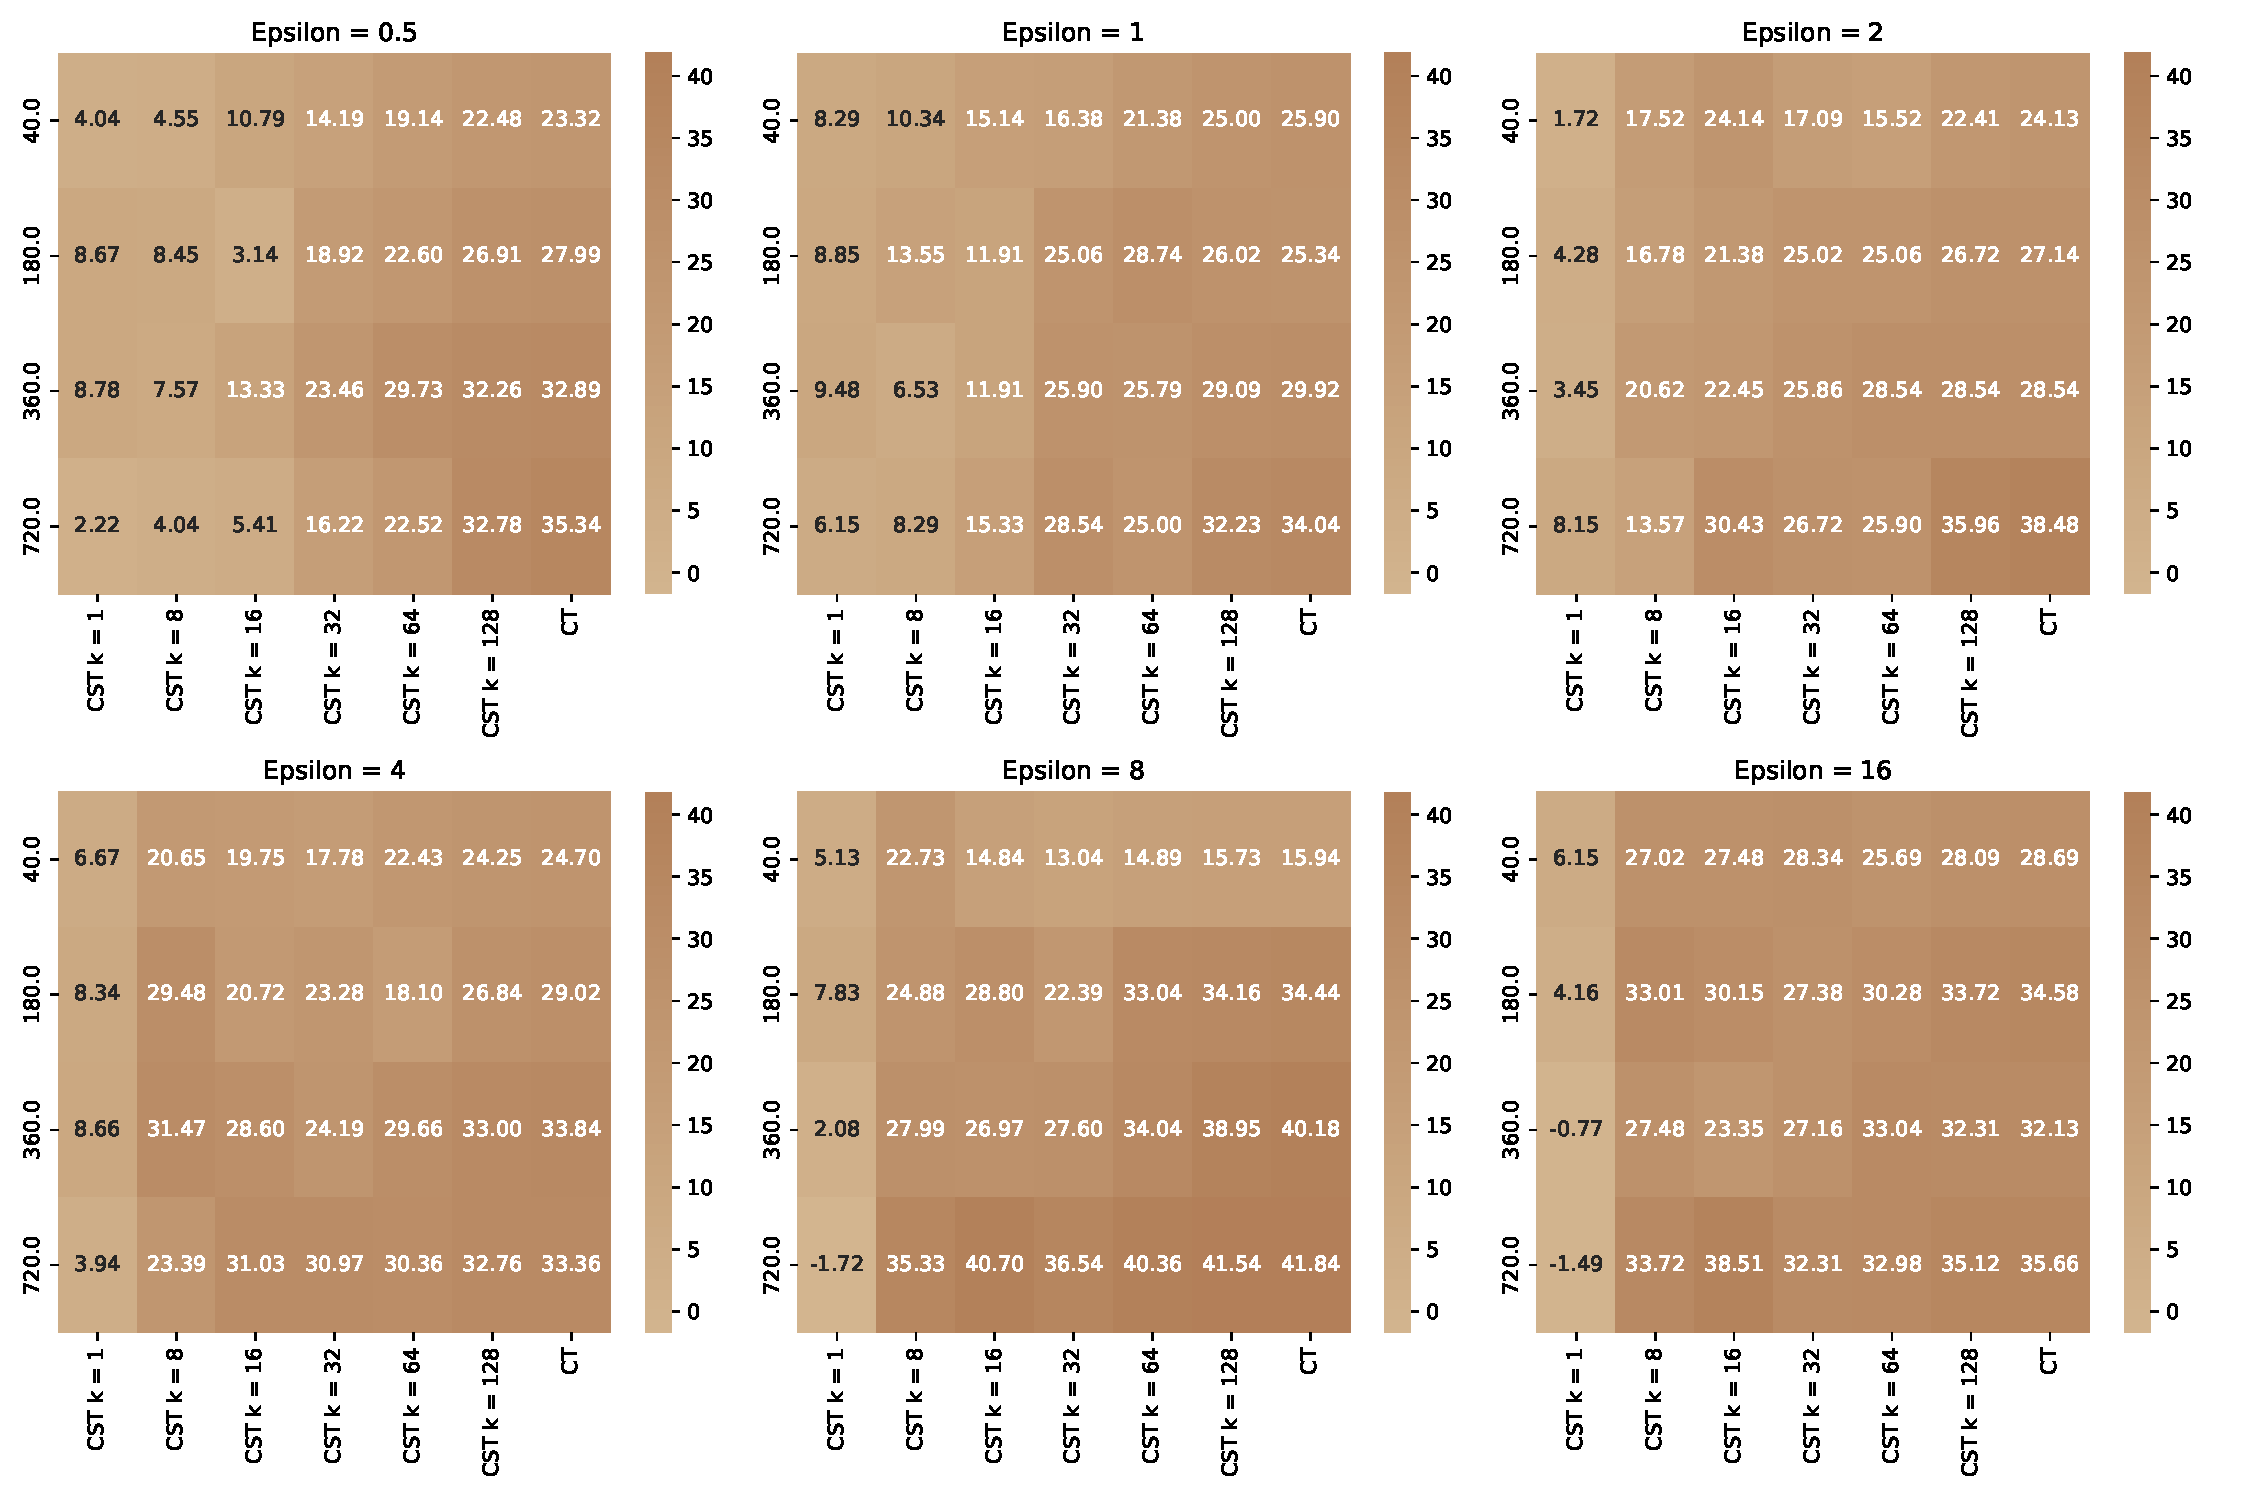
\includegraphics[width=15cm]{latex/fig/heatmap_cohesiveness.pdf}
    \caption{Cohesiveness improvement over SanText (\%); the higher, the better.}
    \label{fig:cohesiveness}
\end{figure*}